% Created 2022-09-15 Thu 12:30
% Intended LaTeX compiler: pdflatex
\documentclass[10pt]{beamer}
\usepackage[utf8]{inputenc}
\usepackage[T1]{fontenc}
\usepackage{graphicx}
\usepackage{longtable}
\usepackage{wrapfig}
\usepackage{rotating}
\usepackage[normalem]{ulem}
\usepackage{amsmath}
\usepackage{amssymb}
\usepackage{capt-of}
\usepackage{hyperref}
\usepackage{minted}
\usepackage{xcolor}
\definecolor{LightGray}{gray}{0.95}
\usefonttheme{professionalfonts}
\setlength{\parskip}{5pt}
\newcommand{\footnoteframe}[1]{\footnote[frame]{#1}}
\addtobeamertemplate{footnote}{}{\vspace{2ex}}
\usepackage{tabularx}
\usepackage{booktabs}
\DefineVerbatimEnvironment{verbatim}{Verbatim}{fontsize=\scriptsize}
\usetheme{Berkeley}
\author{Jay Morgan}
\date{16th September 2022}
\title{Programming Level-up}
\subtitle{Lecture 1 - Introduction and Basic Python Programming}
\hypersetup{
 pdfauthor={Jay Morgan},
 pdftitle={Programming Level-up},
 pdfkeywords={},
 pdfsubject={},
 pdfcreator={Emacs 27.1 (Org mode 9.4.6)}, 
 pdflang={English}}
\begin{document}

\maketitle
\begin{frame}{Outline}
\tableofcontents
\end{frame}


\section{Introduction}
\label{sec:orgf298041}

\subsection{Course introduction}
\label{sec:org39f9319}

\begin{frame}[label={sec:org6249571}]{What\ldots{}? Why\ldots{}?}
\begin{itemize}
\item Programming is much more than the act of programming a small script. Even if you've
programmed before, doing so for a research project requires a lot of rigour to
ensure the results you're reporting are correct, and reproducible.
\item There is so much surrounding the act of programming that it can get a little
overwhelming. Things from setting up a programming environment to managing multiple
experiments on the supercomputers can involve many languages and understanding of
technologies.
\item This course is designed to take you from not being able to program at all to being
able to do it comfortably for your research and work.
\end{itemize}
\end{frame}

\begin{frame}[label={sec:org93d3411}]{What is this course going to teach me?}
\begin{enumerate}
\item Programming with the Python Programming Language.
\begin{itemize}
\item Basic syntax.
\item Introduction to the basics of object oriented programming (OOP).
\item Numerical computing with numpy/pandas/scipy.
\end{itemize}
\item Doing your programming in a Linux-based Environment (GNU/Linux) and being
comfortable with the organisation of this Linux environment.
\begin{itemize}
\item Setting up a research (reproducible) environment.
\item Executing experiments.
\end{itemize}
\item Interacting with the Super-computers/clusters.
\begin{itemize}
\item Interaction with SLURM (management of jobs).
\end{itemize}
\item Taking the results from a program you've created, be able to visualise them and
include them in reports/papers.
\begin{itemize}
\item \LaTeX{}/Markdown.
\item Plotting.
\end{itemize}
\end{enumerate}
\end{frame}

\begin{frame}[label={sec:orgc235782}]{How the course will be delivered}
\begin{itemize}
\item 2/3 hour sessions over the next 2 months.
\item Throughout the lecture, there will be small exercises to try out what we've
learnt. We will go through the answers to these exercises.
\item At the end of the lecture we will have a larger exercise that will become more
challenging. These exercises are not marked, but again, just an opportunity to try
out what you've learnt. The best way to learn how to program is to program.
\end{itemize}
\end{frame}

\begin{frame}[label={sec:org571a182}]{Rough timeline}
\begin{center}
\scriptsize
\begin{tabular}{rll}
\toprule
Lecture & Topic & Description\\
\midrule
1 & Introduction & - Course introduction\\
 &  & - Basic Python programming\\
2 & Python classes & - Introduction to OOP\\
3 & Project management & - Creating/importing modules\\
 &  & - Anaconda/pip\\
4 & Programming environments & - PyCharm\\
 &  & - Jupyter notebooks\\
5 & Numerical computing & - Numpy\\
 &  & - Scipy\\
6 & Numerical computing & - Pandas\\
 &  & - Visualisations\\
7 & Basics of GNU/Linux & - Using the terminal\\
8 & Bash scripting & - Bash scripting\\
9 & High performance computing & - SLURM\\
 &  & - Singularity\\
10 & Reporting & - \LaTeX{}\\
 &  & - Markdown\\
\bottomrule
\end{tabular}
\end{center}
\end{frame}

\subsection{Contact information}
\label{sec:org41ff117}

\begin{frame}[label={sec:orgb72abc9},fragile]{Where to find me}
 My name is Dr Jay Morgan. I am a researcher work on Deep Learning in Astrophysics.

\begin{itemize}
\item Email: \texttt{jay.morgan@univ-tln.fr}
\item Lecture slides and other contact on my website: \url{https://pageperso.lis-lab.fr/jay.morgan/}
\end{itemize}

\begin{center}

\includegraphics[width=0.5\textwidth]{./images/website.png}
\end{center}
\end{frame}

\section{Python}
\label{sec:org81d6e21}

\subsection{Introducing Python}
\label{sec:orgab38537}

\begin{frame}[label={sec:orgd3b1c69}]{Python}
\begin{center}
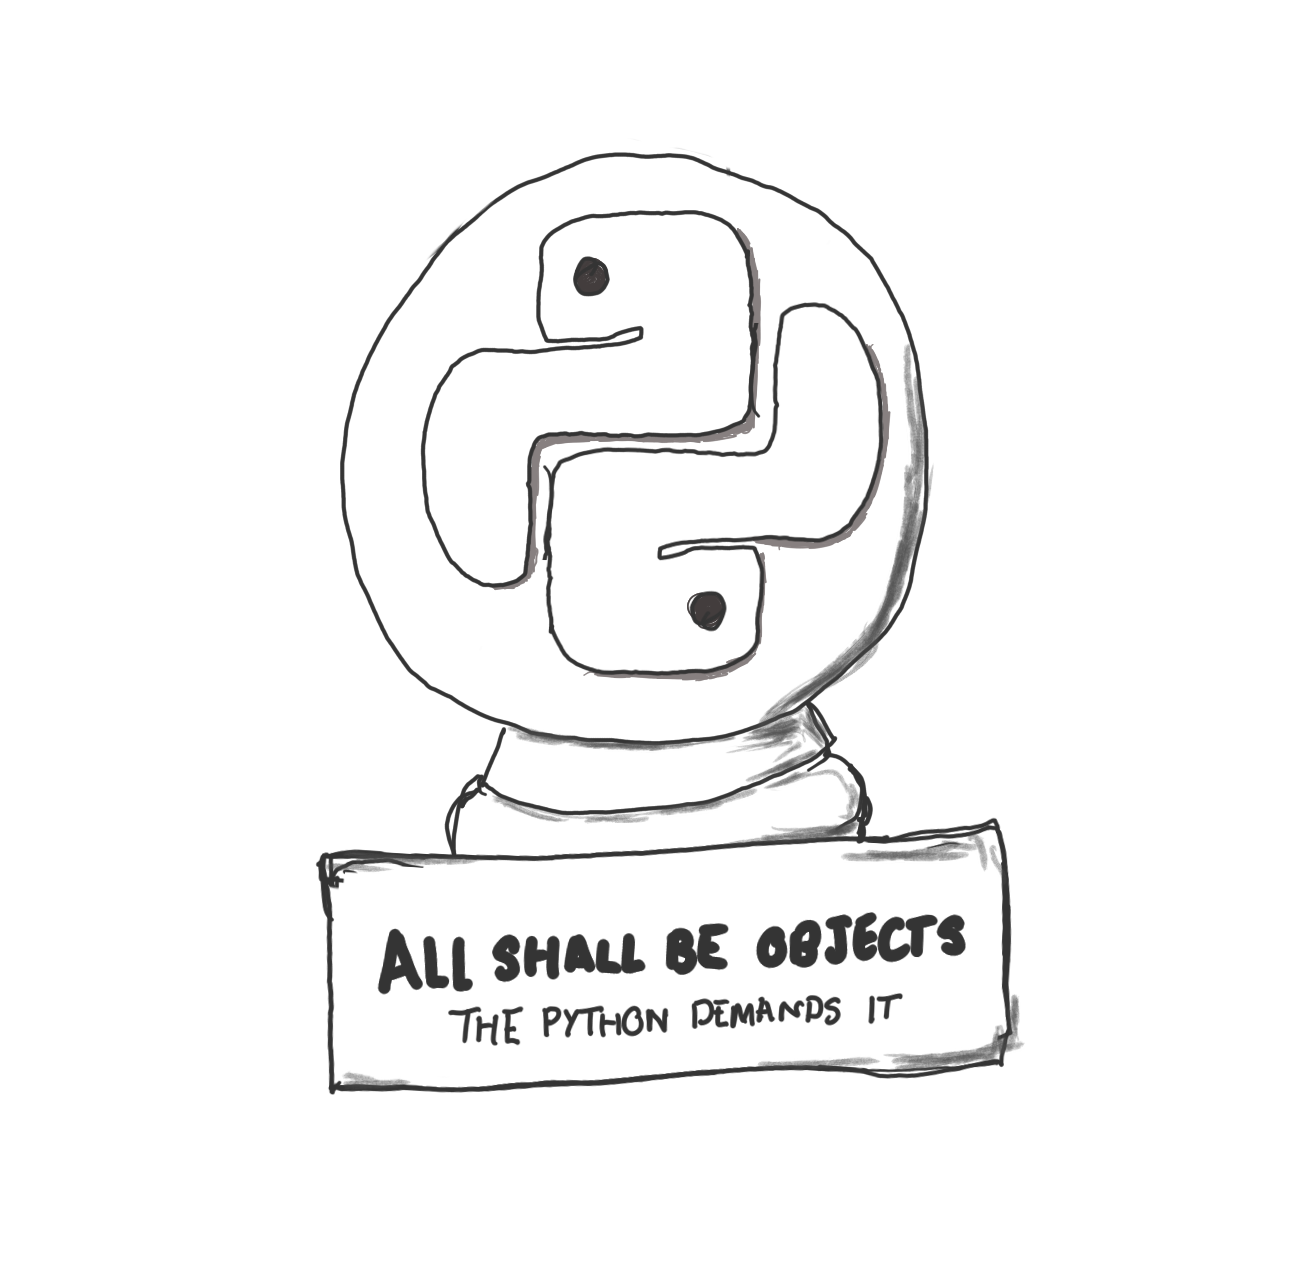
\includegraphics[width=0.7\textwidth]{./images/python-objects.png}
\end{center}
\end{frame}

\begin{frame}[label={sec:orgf12785c}]{Python}
\begin{columns}
\begin{column}{0.6\columnwidth}
\begin{itemize}
\item Python is a \emph{high-level}\footnoteframe{As we go through our lectures we'll understand what it means for the language to be /high-level/ and /interpreted/ and why that is helpful for us.} programming language created in 1991.
\item While it is an old language, its become vastly popular thanks to its use in data
science and other mathematics-based disciplines. While also being able to perform
tasks such as GUI, web-development and much more.
\item Because the language is high-level and \emph{interpreted}, programmers can often find
themselves more productive in Python than in other languages such as say C++.
\end{itemize}
\end{column}

\begin{column}{0.3\columnwidth}
\begin{center}
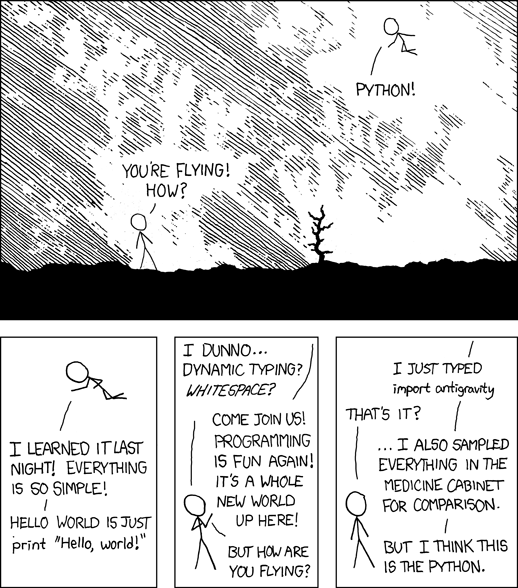
\includegraphics[width=\textwidth]{./images/python.png}
\end{center}
\end{column}
\end{columns}
\end{frame}


\begin{frame}[label={sec:orgff6fb78},fragile]{A first program}
 We're going to start with the 'Hello, World' program that prints \texttt{Hello, World!} to the
screen. In python this is as simple as writing:

\begin{minted}[frame=lines,linenos=true,firstnumber=last,fontsize=\footnotesize,bgcolor=LightGray,xleftmargin=5pt,tabsize=2,breaklines=true,numbersep=10pt]{python}
print("Hello, World!")   # this prints: Hello, World!
\end{minted}

\begin{verbatim}
Results: 
# => Hello, World!
\end{verbatim}


\alert{NOTE} anything following a \texttt{\#} is a comment and is completely ignored by the
computer. It is there for you to document your code for others, and most
importantly, for yourself.
\end{frame}

\begin{frame}[label={sec:org3b35d04},fragile]{Running this program}
 Before we can run this program, we need to save it somewhere. For this, will
create a new file, insert this text, and save it as \texttt{<filename>.py}, where
\texttt{<filename>} is what we want to call the script. This name doesn't matter for its
execution.

Once we have created the \emph{script}, we can run it from the \emph{command line}. We will
get into the command line in a later lecture, but right now all you need to know
is:

\begin{minted}[frame=lines,linenos=true,firstnumber=last,fontsize=\footnotesize,bgcolor=LightGray,xleftmargin=5pt,tabsize=2,breaklines=true,numbersep=10pt]{bash}
python3 <filename>.py
\end{minted}
\end{frame}

\begin{frame}[label={sec:org8e48dfa},fragile]{An alternative method of running python}
 You may notice that if you don't give \texttt{python} a filename to run, you will enter
something called the \texttt{REPL}.

\begin{minted}[frame=lines,linenos=true,firstnumber=last,fontsize=\footnotesize,bgcolor=LightGray,xleftmargin=5pt,tabsize=2,breaklines=true,numbersep=10pt]{bash}
Python 3.9.5 (default, Jun  4 2021, 12:28:51) 
[GCC 7.5.0] :: Anaconda, Inc. on linux
Type "help", "copyright", "credits" or "license" for more information.
>>> 
\end{minted}

\texttt{REPL} stands for \texttt{READ}, \texttt{EXECUTE}, \texttt{PRINT}, \texttt{LOOP}.
\end{frame}

\begin{frame}[label={sec:org14f39ff},fragile]{Variables}
 A \emph{variable} is a \emph{symbol} associated with a \emph{value}. This value can differ widely, and we
will take a look at different types of values/data later.

Neverthless, variables are useful for \emph{referring} to values and \emph{storing} to the results
of a computation.

\begin{minted}[frame=lines,linenos=true,firstnumber=last,fontsize=\footnotesize,bgcolor=LightGray,xleftmargin=5pt,tabsize=2,breaklines=true,numbersep=10pt]{python}
x = 1
y = 2
z = x + y
print(z)   # prints: 3

# variables can be /overwritten/
z = "hello, world"
print(z)   # prints: hello, world
\end{minted}

\begin{verbatim}
Results: 
# => 3
# => hello, world
\end{verbatim}
\end{frame}

\subsection{Types of data}
\label{sec:org595ee05}

\begin{frame}[label={sec:org34e41d5},fragile]{Primitive data types}
 Primitive data types are the most fundamental parts of programming, they cannot
be \emph{broken} down.

\begin{minted}[frame=lines,linenos=true,firstnumber=last,fontsize=\footnotesize,bgcolor=LightGray,xleftmargin=5pt,tabsize=2,breaklines=true,numbersep=10pt]{python}
"Hello" # string
1       # integer
1.0     # float
True    # Boolean (or bool for short)
\end{minted}
\end{frame}

\begin{frame}[label={sec:org3ab19aa},fragile]{Primitive data type}
 We can get the type of some data by using the \texttt{type(...)} function. For example,

\begin{minted}[frame=lines,linenos=true,firstnumber=last,fontsize=\footnotesize,bgcolor=LightGray,xleftmargin=5pt,tabsize=2,breaklines=true,numbersep=10pt]{python}
print(type(5))
print(type(5.0))

x = "all cats meow"

print(type(x))
\end{minted}

\begin{verbatim}
Results: 
# => <class 'int'>
# => <class 'float'>
# => <class 'str'>
\end{verbatim}
\end{frame}

\begin{frame}[label={sec:org6921939},fragile]{Basic Math with primitives}
 Using these primitive data types, we can do some basic math operations!

\begin{minted}[frame=lines,linenos=true,firstnumber=last,fontsize=\footnotesize,bgcolor=LightGray,xleftmargin=5pt,tabsize=2,breaklines=true,numbersep=10pt]{python}
print(1 + 2)    # Addtion
print(1 - 2)    # Subtraction
print(1 * 2)    # Multiplication
print(1 / 2)    # Division
print(2 ** 2)   # Exponent
print(3 % 2)    # Modulo operator
\end{minted}

\begin{verbatim}
Results: 
# => 3
# => -1
# => 2
# => 0.5
# => 4
# => 1
\end{verbatim}
\end{frame}

\begin{frame}[label={sec:org7e8de7a},fragile]{Basic Math}
 Sometimes types get converted to the same type:

\begin{minted}[frame=lines,linenos=true,firstnumber=last,fontsize=\footnotesize,bgcolor=LightGray,xleftmargin=5pt,tabsize=2,breaklines=true,numbersep=10pt]{python}
print(1.0 + 2)  # float + integer = float
\end{minted}

\begin{verbatim}
Results: 
# => 3.0
\end{verbatim}


Even more interesting is with Booleans!

\begin{minted}[frame=lines,linenos=true,firstnumber=last,fontsize=\footnotesize,bgcolor=LightGray,xleftmargin=5pt,tabsize=2,breaklines=true,numbersep=10pt]{python}
True + True
\end{minted}

\begin{verbatim}
Results: 
# => 2
\end{verbatim}
\end{frame}

\begin{frame}[label={sec:org9d95d7a},fragile]{BODMAS in Python}
 Like in mathematics, certain math operator take precedence over others.

\begin{itemize}
\item B - Brackets
\item O - Orders (roots, exponents)
\item D - division
\item M - multiplication
\item A - addition
\item S - subtraction.
\end{itemize}

To make the context clear as to what operations to perform first, use brackets.

\begin{minted}[frame=lines,linenos=true,firstnumber=last,fontsize=\footnotesize,bgcolor=LightGray,xleftmargin=5pt,tabsize=2,breaklines=true,numbersep=10pt]{python}
(5 / 5) + 1
5 / (5 + 1)
\end{minted}

\begin{verbatim}
Results: 
# => 2.0
# => 0.8333333333333334
\end{verbatim}
\end{frame}

\begin{frame}[label={sec:orge949981},fragile]{Basic Math -- Quick exercise}
 Write the following equation in python:

\((5 + 2) \times (\frac{10}{2} + 10)^2\)

\alert{Remember} to use parentheses \texttt{( )} to ensure that operations take precedence over
others.

Your answer should come out as: \texttt{1575.0}
\end{frame}

\subsection{Working with strings}
\label{sec:org1525e19}

\begin{frame}[label={sec:org4b1d699},fragile]{Formatting strings}
 In many previous examples when we've printed strings, we've done something like:

\begin{minted}[frame=lines,linenos=true,firstnumber=last,fontsize=\footnotesize,bgcolor=LightGray,xleftmargin=5pt,tabsize=2,breaklines=true,numbersep=10pt]{python}
age = 35

print("The value of age is", age)
\end{minted}

\begin{verbatim}
Results: 
# => The value of age is 35
\end{verbatim}


While this works in this small context, it can get pretty cumbersome if we have many
variables we want to print, and we also want to change how they are displayed when
they are printed.

We're going to take a look now at much better ways of printing.
\end{frame}

\begin{frame}[label={sec:orga48d893},fragile]{Better ways of printing strings - \%}
 The first method is using \texttt{\%}. When we print, we first construct a string with special
delimiters, such as \texttt{\%s} that denotes a string, and \texttt{\%d} that denotes a number. This is
telling Python where we want the values to be placed in the string.

Once we've created the string, we need to specify the data, which we do with \texttt{\%
(...)}. Like, for example:

\begin{minted}[frame=lines,linenos=true,firstnumber=last,fontsize=\footnotesize,bgcolor=LightGray,xleftmargin=5pt,tabsize=2,breaklines=true,numbersep=10pt]{python}
age = 35
name = "John"

print("%d years old" % age)  # no tuple for one variable
print("%s is %d years old" % (name, age)) 
\end{minted}

\begin{verbatim}
Results: 
# => 35 years old
# => John is 35 years old
\end{verbatim}


Here we are specifying the a string \texttt{\%s} and number \texttt{\%d}, and then giving the variables
that correspond with that data type.
\end{frame}

\begin{frame}[label={sec:org2fdcd2f},fragile]{Better ways of printing strings -- data specifiers}
 The special delimiters correspond with a data type. Here are some of the most common:

\begin{itemize}
\item \texttt{\%s} -- For strings
\item \texttt{\%d} -- For numbers
\item \texttt{\%f} -- For floating point numbers.
\end{itemize}

There are others such as \texttt{\%x} that prints the hexadecimal representation, but these are
less common. You can find the full list at: \url{https://docs.python.org/3/library/stdtypes.html\#old-string-formatting}
\end{frame}

\begin{frame}[label={sec:orge1b6018},fragile]{Better ways of printing strings -- floating points}
 When using these delimiters, we can add modifiers to how they format and display the
value. Take a very common example, where we have a floating point value, and, when
printing it, we only want to print to 3 decimal places. To accomplish this, we again
use \texttt{\%f} but add a \texttt{.3} to between the \texttt{\%} and \texttt{f}. In this example, we are printing \(\pi\) to 3
decimal places.

\begin{minted}[frame=lines,linenos=true,firstnumber=last,fontsize=\footnotesize,bgcolor=LightGray,xleftmargin=5pt,tabsize=2,breaklines=true,numbersep=10pt]{python}
print("Pi to 3 digits is: %.3f" % 3.1415926535)
\end{minted}

\begin{verbatim}
Results: 
# => Pi to 3 digits is: 3.142
\end{verbatim}
\end{frame}

\begin{frame}[label={sec:orgad0c67e},fragile]{Better ways of printing strings -- floating points}
 In the previous example, we used \texttt{.3} to specify 3 decimal places. If we put a number
before the decimal, like \texttt{10.3} we are telling Python \emph{make this float occupy 10 spaces
and this float should have 3 decimal places printed}.  When it gets printed, you will
notice that it shifts to the right, it gets padded by space. If we use a negative
number in front of the decimal place, we are telling python to shift it to the left.

\begin{minted}[frame=lines,linenos=true,firstnumber=last,fontsize=\footnotesize,bgcolor=LightGray,xleftmargin=5pt,tabsize=2,breaklines=true,numbersep=10pt]{python}
print("Pi to 3 digits is: %10.3f" % 3.1415926535)
print("Pi to 3 digits is: %-10.3f" % 3.1415926535)
\end{minted}

\begin{verbatim}
Results: 
# => Pi to 3 digits is:      3.142
# => Pi to 3 digits is: 3.142
\end{verbatim}
\end{frame}

\begin{frame}[label={sec:orga1f96c0},fragile]{Better ways of printing strings -- \texttt{f-strings}}
 The final method of formatting strings is a newcomer within the language, it is the
so-called \texttt{f-string}. Where a \texttt{f} character is prefixed to the beginning of the string
you're creating. \texttt{f-string}'s allow you to use Python syntax within the string (again
delimited by \texttt{\{\}}.

Take this for example where we are referencing the variables \texttt{name} and \texttt{age} directly.

\begin{minted}[frame=lines,linenos=true,firstnumber=last,fontsize=\footnotesize,bgcolor=LightGray,xleftmargin=5pt,tabsize=2,breaklines=true,numbersep=10pt]{python}
name = "Jane"
age = 35

print(f"{name} is {age} years old")
\end{minted}

\begin{verbatim}
Results: 
# => Jane is 35 years old
\end{verbatim}
\end{frame}

\begin{frame}[label={sec:org363b178},fragile]{Better ways of printing strings -- \texttt{f-strings}}
 \texttt{f-string}'s allow you to execute Python code within the string. Here we are accessing
the value from the dictionary by specifying the key within the string itself! It
certainly makes it a lot easier, especially if we only need to access the values for
the string itself.

\begin{minted}[frame=lines,linenos=true,firstnumber=last,fontsize=\footnotesize,bgcolor=LightGray,xleftmargin=5pt,tabsize=2,breaklines=true,numbersep=10pt]{python}
contact_info = {"name": "Jane", "age": 35}

print(f"{contact_info['name']} is {contact_info['age']} years old")
\end{minted}

\begin{verbatim}
Results: 
# => Jane is 35 years old
\end{verbatim}


\url{https://pyformat.info/}
\end{frame}

\begin{frame}[label={sec:org524dc95},fragile]{Better ways of printing strings -- \texttt{f-string}}
 We can still format the values when using \texttt{f-string}. The method is similar to those
using the \texttt{\%f} specifiers.

\begin{minted}[frame=lines,linenos=true,firstnumber=last,fontsize=\footnotesize,bgcolor=LightGray,xleftmargin=5pt,tabsize=2,breaklines=true,numbersep=10pt]{python}
pi = 3.1415926535
print(f"Pi is {pi:.3f} to 3 decimal places")
\end{minted}

\begin{verbatim}
Results: 
# => Pi is 3.142 to 3 decimal places
\end{verbatim}


Many more examples can be found at: \url{https://zetcode.com/python/fstring/}
\end{frame}

\begin{frame}[label={sec:org178f7bf},fragile]{Operations on strings -- splitting}
 Apart from formatting, there are plenty more operations we can perform on strings. We
are going to highlight some of the most common here.

The first we're going to look at is splitting a string by a delimiter character using
the \texttt{.split()} method. If we don't pass any argument to the \texttt{.split()} method, then by
default, it will split by spaces. However, we can change this by specifying the
delimiter.

\begin{minted}[frame=lines,linenos=true,firstnumber=last,fontsize=\footnotesize,bgcolor=LightGray,xleftmargin=5pt,tabsize=2,breaklines=true,numbersep=10pt]{python}
my_string = "This is a sentence, where each word is separated by a space"

print(my_string.split())
print(my_string.split(","))
\end{minted}

\begin{verbatim}
Results: 
# => ['This', 'is', 'a', 'sentence,', 'where', 'each', 'word', 'is', 'separated', 'by', 'a', 'space']
# => ['This is a sentence', ' where each word is separated by a space']
\end{verbatim}
\end{frame}

\begin{frame}[label={sec:orgdf51cbd},fragile]{Operations on strings -- joining}
 As \texttt{.split()} splits a single string into a list, \texttt{.join()} joins a list of strings into
a single string. To use \texttt{.join()}, we first create a string of the delimiter we want to
use to join the list of strings by. In this example we're going to use \texttt{"-"}. Then we
call the \texttt{.join()} method, passing the list as an argument.

The result is a single string using the delimiter to separate the items of the list.

\begin{minted}[frame=lines,linenos=true,firstnumber=last,fontsize=\footnotesize,bgcolor=LightGray,xleftmargin=5pt,tabsize=2,breaklines=true,numbersep=10pt]{python}
x = ['This', 'is', 'a', 'sentence,', 'where', 'each', 'word', 'is', 'separated', 'by', 'a', 'space']

print("-".join(x))
\end{minted}

\begin{verbatim}
Results: 
# => This-is-a-sentence,-where-each-word-is-separated-by-a-space
\end{verbatim}
\end{frame}

\begin{frame}[label={sec:orgbf6af11},fragile]{Operations on strings -- changing case}
 Other common operations on strings involve change the case. For example:

\begin{itemize}
\item Make the entire string uppercase or lowercase
\item Making the string title case (every where starts with a capital letter).
\item Stripping the string by removing any empty spaces either side of the string.
\end{itemize}

\alert{Note} we can chain many methods together by doing \texttt{.method\_1().method\_2()}, but only if they
return string. If they return \texttt{None}, then chaining will not work.

\begin{minted}[frame=lines,linenos=true,firstnumber=last,fontsize=\footnotesize,bgcolor=LightGray,xleftmargin=5pt,tabsize=2,breaklines=true,numbersep=10pt]{python}
x = "    this String Can change case"

print(x.upper())
print(x.lower())
print(x.title())
print(x.strip())
print(x.strip().title())
\end{minted}

\begin{verbatim}
Results: 
# =>     THIS STRING CAN CHANGE CASE
# =>     this string can change case
# =>     This String Can Change Case
# => this String Can change case
# => This String Can Change Case
\end{verbatim}
\end{frame}

\begin{frame}[label={sec:org212bcea},fragile]{Operations on strings -- replacing strings}
 To replace a substring, we use the \texttt{.replace()} method. The first argument is the old
string you want to replace. The second argument is what you want to replace it with.

\begin{minted}[frame=lines,linenos=true,firstnumber=last,fontsize=\footnotesize,bgcolor=LightGray,xleftmargin=5pt,tabsize=2,breaklines=true,numbersep=10pt]{python}
x = "This is a string that contains some text"

print(x.replace("contains some", "definitely contains some"))
\end{minted}

\begin{verbatim}
Results: 
# => This is a string that definitely contains some text
\end{verbatim}
\end{frame}

\subsection{Compound data structures}
\label{sec:org3e69100}
\begin{frame}[label={sec:orgf746875},fragile]{Container data types/Data structures}
 Container data types or data structures, as the name suggests, are used to contain
other things. Types of containers are:

\begin{itemize}
\item Lists
\item Dictionaries
\item Tuples
\item Sets
\end{itemize}

\begin{minted}[frame=lines,linenos=true,firstnumber=last,fontsize=\footnotesize,bgcolor=LightGray,xleftmargin=5pt,tabsize=2,breaklines=true,numbersep=10pt]{python}
[1, "hello", 2]                 # list
{"my-key": 2, "your-key": 1}    # dictionary (or dict)
(1, 2)                          # tuple
set(1, 2)                       # set
\end{minted}

We'll take a look at each of these different container types and explore why we
might want to use each of them.
\end{frame}

\begin{frame}[label={sec:org7ad1782},fragile]{An aside on Terminology}
 To make our explanations clearer and reduce confusion, each of the different symbols
have unique names.

I will use this terminology consistently throughout the course, and it is common to
see the same use outside the course.

\begin{itemize}
\item \texttt{[ ]} brackets (square brackets).
\item \texttt{\{ \}} braces (curly braces).
\item \texttt{( )} parentheses.
\end{itemize}
\end{frame}

\begin{frame}[label={sec:org96cffb3},fragile]{Lists}
 A hetreogenious container. This means that it can store any type of data.

\begin{minted}[frame=lines,linenos=true,firstnumber=last,fontsize=\footnotesize,bgcolor=LightGray,xleftmargin=5pt,tabsize=2,breaklines=true,numbersep=10pt]{python}
x = [1, "hello", 2]
\end{minted}

Elements can be accessed using indexing \texttt{[ ]} notation. For example:

\begin{minted}[frame=lines,linenos=true,firstnumber=last,fontsize=\footnotesize,bgcolor=LightGray,xleftmargin=5pt,tabsize=2,breaklines=true,numbersep=10pt]{python}
print(x[0])    # this will get the first element (i.e. 1)
print(x[1])    # the second element (i.e. "hello")
print(x[2])    # the third element (i.e. 2)
\end{minted}

\begin{verbatim}
Results: 
# => 1
# => hello
# => 2
\end{verbatim}


\alert{notice how the first element is the 0-th item in the list/} we say that python is
0-indexed.
\end{frame}

\begin{frame}[label={sec:orgf8b4e1c},fragile]{Better indexing -- slices}
 If we wanted to access an element from a data structure, such as a list, we would use
the \texttt{[ ]} accessor, specifying the index of the element we wish to retrieve (remember
that indexes start at zero!). But what if we ranted to access many elements at once?
Well to accomplish that, we have a slice or a range of indexes (not to be confused
with the \texttt{range} function). A slice is defined as:

\begin{verbatim}
start_index:end_index
\end{verbatim}

where the \texttt{end\_index} is non inclusive -- it doesn't get included in the result. Here
is an example where we have a list of 6 numbers from 0 to 5, and we slice the list from index
0 to 3. Notice how the 3rd index is not included.

\begin{minted}[frame=lines,linenos=true,firstnumber=last,fontsize=\footnotesize,bgcolor=LightGray,xleftmargin=5pt,tabsize=2,breaklines=true,numbersep=10pt]{python}
x = [0, 1, 2, 3, 4, 5]
print(x[0:3])
\end{minted}

\begin{verbatim}
Results: 
# => [0, 1, 2]
\end{verbatim}
\end{frame}

\begin{frame}[label={sec:org11c8435},fragile]{Better indexing -- range}
 When we use \texttt{start\_index:end\_index}, the slice increments by 1 from \texttt{start\_index} to
\texttt{end\_index}. If we wanted to increment by a different amount we can use the slicing
form:

\begin{verbatim}
start_index:end_index:step
\end{verbatim}

Here is an example where we step the indexes by 2:

\begin{minted}[frame=lines,linenos=true,firstnumber=last,fontsize=\footnotesize,bgcolor=LightGray,xleftmargin=5pt,tabsize=2,breaklines=true,numbersep=10pt]{python}
x = list(range(100))
print(x[10:15:2])
\end{minted}

\begin{verbatim}
Results: 
# => [10, 12, 14]
\end{verbatim}
\end{frame}

\begin{frame}[label={sec:org1d191ba},fragile]{Better indexing -- reverse}
 One strange fact about the step is that if we specify a negative number for the step,
Python will work backwards, and effectively reverse the list.

\begin{minted}[frame=lines,linenos=true,firstnumber=last,fontsize=\footnotesize,bgcolor=LightGray,xleftmargin=5pt,tabsize=2,breaklines=true,numbersep=10pt]{python}
x = list(range(5))

print(x[::-1])
\end{minted}

\begin{verbatim}
Results: 
# => [4, 3, 2, 1, 0]
\end{verbatim}
\end{frame}

\begin{frame}[label={sec:org76fa54c},fragile]{Better indexing -- range}
 In a previous example, I created a slice like \texttt{0:3}. This was a little wasteful as we
can write slightly less code. If we write \texttt{:end\_index}, Python assumes and creates a
slice from the first index (0) to the \texttt{end\_index}. If we write \texttt{start\_index:}, Python
assumes and creates a slice from \texttt{start\_index} to the end of the list.

\begin{minted}[frame=lines,linenos=true,firstnumber=last,fontsize=\footnotesize,bgcolor=LightGray,xleftmargin=5pt,tabsize=2,breaklines=true,numbersep=10pt]{python}
x = list(range(100))

print(x[:10])
print(x[90:])
\end{minted}

\begin{verbatim}
Results: 
# => [0, 1, 2, 3, 4, 5, 6, 7, 8, 9]
# => [90, 91, 92, 93, 94, 95, 96, 97, 98, 99]
\end{verbatim}
\end{frame}

\begin{frame}[label={sec:org048b51c},fragile]{Better indexing -- backwards}
 Finally, we also work backwards from the end of list. If we use a negative number,
such as -1, we are telling Python, take the elements from the end of the list. -1 is
the final index, and numbers lower than -1 work further backwards through the list.

\begin{minted}[frame=lines,linenos=true,firstnumber=last,fontsize=\footnotesize,bgcolor=LightGray,xleftmargin=5pt,tabsize=2,breaklines=true,numbersep=10pt]{python}
x = list(range(100))

print(x[-1])
print(x[-2])
\end{minted}

\begin{verbatim}
Results: 
# => 99
# => 98
\end{verbatim}
\end{frame}

\begin{frame}[label={sec:org74f74d9},fragile]{Better indexing --backwards}
 Slicing with negative indexes, also works. Here we are creating a slice from the end
of the list - 10, to the last (but not including) index.

\begin{minted}[frame=lines,linenos=true,firstnumber=last,fontsize=\footnotesize,bgcolor=LightGray,xleftmargin=5pt,tabsize=2,breaklines=true,numbersep=10pt]{python}
x = list(range(100))

print(x[-10:-1])
\end{minted}

\begin{verbatim}
Results: 
# => [90, 91, 92, 93, 94, 95, 96, 97, 98]
\end{verbatim}
\end{frame}

\begin{frame}[label={sec:org26de6ee},fragile]{Lists -- adding data}
 If we want to add items to the end of the list, we use the \texttt{append} function:

\begin{minted}[frame=lines,linenos=true,firstnumber=last,fontsize=\footnotesize,bgcolor=LightGray,xleftmargin=5pt,tabsize=2,breaklines=true,numbersep=10pt]{python}
my_list = []

my_list.append("all")
my_list.append("dogs")
my_list.append("bark")

print(my_list)
\end{minted}

\begin{verbatim}
Results: 
# => ['all', 'dogs', 'bark']
\end{verbatim}
\end{frame}

\begin{frame}[label={sec:orge6bbc81},fragile]{Dictionaries}
 Dictionaries are a little different from lists as each 'element' consists of a
key-pair value. Let's have a look at some examples where the dictionaries contains
\alert{one} element:

\begin{minted}[frame=lines,linenos=true,firstnumber=last,fontsize=\footnotesize,bgcolor=LightGray,xleftmargin=5pt,tabsize=2,breaklines=true,numbersep=10pt]{python}
my_dictionary = {"key": "value"}
my_other_dict = {"age": 25}
\end{minted}

To access the \emph{value}, we get it using \texttt{[key]} notation:

\begin{minted}[frame=lines,linenos=true,firstnumber=last,fontsize=\footnotesize,bgcolor=LightGray,xleftmargin=5pt,tabsize=2,breaklines=true,numbersep=10pt]{python}
my_other_dict["age"]
\end{minted}

\begin{verbatim}
Results: 
# => 25
\end{verbatim}


\alert{NOTE} keys are unique, i.e:

\begin{minted}[frame=lines,linenos=true,firstnumber=last,fontsize=\footnotesize,bgcolor=LightGray,xleftmargin=5pt,tabsize=2,breaklines=true,numbersep=10pt]{python}
my_dictionary = {"age": 25, "age": 15}
my_dictionary["age"]
\end{minted}

\begin{verbatim}
Results: 
# => 15
\end{verbatim}
\end{frame}

\begin{frame}[label={sec:orgbff2767},fragile]{Dictionaries}
 The key in the dictionary doesn't necessarily need to be a string. For example, in
this case, we have created two key-pair elements, where the keys to both are tuples
of numbers.

\begin{minted}[frame=lines,linenos=true,firstnumber=last,fontsize=\footnotesize,bgcolor=LightGray,xleftmargin=5pt,tabsize=2,breaklines=true,numbersep=10pt]{python}
my_dictionary = {(1, 2): "square", (3, 4): "circle"}

print(my_dictionary[(1, 2)])
\end{minted}

\begin{verbatim}
Results: 
# => square
\end{verbatim}
\end{frame}

\begin{frame}[label={sec:org272130b},fragile]{Dictionaries -- adding data}
 If we want to add data to a dictionary, we simply perform the accessor method with a
key that is not in the dictionary:

\begin{minted}[frame=lines,linenos=true,firstnumber=last,fontsize=\footnotesize,bgcolor=LightGray,xleftmargin=5pt,tabsize=2,breaklines=true,numbersep=10pt]{python}
my_dict = {}

my_dict["name"] = "James"
my_dict["age"] = 35

print(my_dict)
\end{minted}

\begin{verbatim}
Results: 
# => {'name': 'James', 'age': 35}
\end{verbatim}
\end{frame}

\begin{frame}[label={sec:orge3644a8},fragile]{Dictionaries -- Quick Exercise}
 \begin{itemize}
\item Create a dictionary for the following address, and assign it a variable name
called \texttt{address}:
\end{itemize}

\begin{center}
\begin{tabular}{ll}
\toprule
Key & Value\\
\midrule
number & 22\\
street & Bakers Street\\
city & London\\
\bottomrule
\end{tabular}
\end{center}

\begin{itemize}
\item Print out the address's street name using the \texttt{[ ]} accessor with the correct key.
\end{itemize}
\end{frame}

\begin{frame}[label={sec:orgce99ae0},fragile]{Tuples}
 \begin{minted}[frame=lines,linenos=true,firstnumber=last,fontsize=\footnotesize,bgcolor=LightGray,xleftmargin=5pt,tabsize=2,breaklines=true,numbersep=10pt]{python}
my_tuple = (1, 56, -2)
\end{minted}

Like lists, elements of the tuple can be accessed by their position in the list,
starting with the 0-th element:

\begin{minted}[frame=lines,linenos=true,firstnumber=last,fontsize=\footnotesize,bgcolor=LightGray,xleftmargin=5pt,tabsize=2,breaklines=true,numbersep=10pt]{python}
print(my_tuple[0])  # => 1
print(my_tuple[1])  # => 56
print(my_tuple[2])  # => -2
\end{minted}

\begin{verbatim}
Results: 
# => 1
# => 56
# => -2
\end{verbatim}
\end{frame}

\begin{frame}[label={sec:org417eed5},fragile]{Tuples}
 Unlike lists, tuples cannot be changed after they've been created. We say they are
\alert{immutable}. So this will \alert{not} work:

\begin{minted}[frame=lines,linenos=true,firstnumber=last,fontsize=\footnotesize,bgcolor=LightGray,xleftmargin=5pt,tabsize=2,breaklines=true,numbersep=10pt]{python}
my_tuple[2] = "dogs"  # creates an Error
\end{minted}

\begin{verbatim}
Results: 
# => Traceback (most recent call last):
  File "<stdin>", line 1, in <module>
  File "/tmp/pyKdIIcx", line 18, in <module>
  File "<string>", line 1, in <module>
TypeError: 'tuple' object does not support item assignment
\end{verbatim}
\end{frame}

\begin{frame}[label={sec:org305e24c},fragile]{Sets}
 Sets in Python are like tuples, but contain only unique elements.

You can use the \texttt{set( )} function (\alert{more on functions later!}), supplying a list, to create a set:

\begin{minted}[frame=lines,linenos=true,firstnumber=last,fontsize=\footnotesize,bgcolor=LightGray,xleftmargin=5pt,tabsize=2,breaklines=true,numbersep=10pt]{python}
my_set = set([1, 2, 2, 2, 3, 4])
my_set
\end{minted}

\begin{verbatim}
Results: 
# => {1, 2, 3, 4}
\end{verbatim}


Notice how there is only one '2' in the resulting set, duplicate elements are removed.
\end{frame}

\begin{frame}[label={sec:org4ce8bb4},fragile]{Sets -- adding data}
 If we want to add data to a set, we use the \texttt{.add()} method. The element used as an
argument to this function will only be added to the set if it is not already in the
set.

\begin{minted}[frame=lines,linenos=true,firstnumber=last,fontsize=\footnotesize,bgcolor=LightGray,xleftmargin=5pt,tabsize=2,breaklines=true,numbersep=10pt]{python}
my_set = set([])

my_set.add(1)
my_set.add(2)
my_set.add(1)

print(my_set)
\end{minted}

\begin{verbatim}
Results: 
# => {1, 2}
\end{verbatim}
\end{frame}

\subsection{Conditional expressions}
\label{sec:org271618c}
\begin{frame}[label={sec:org8812c40},fragile]{If statement}
 If statements allow for branching paths of execution. In other words, we can execute
some statements if some conditions holds (or does not hold).

The structure of a simple if statement is:

\begin{minted}[frame=lines,linenos=true,firstnumber=last,fontsize=\footnotesize,bgcolor=LightGray,xleftmargin=5pt,tabsize=2,breaklines=true,numbersep=10pt]{python}
if <condition>:
    <body>
\end{minted}

\begin{minted}[frame=lines,linenos=true,firstnumber=last,fontsize=\footnotesize,bgcolor=LightGray,xleftmargin=5pt,tabsize=2,breaklines=true,numbersep=10pt]{python}
x = 2
y = "stop"

if x < 5:
    print("X is less than five")
if y == "go":
    print("All systems go!!")
\end{minted}

\begin{verbatim}
Results: 
# => X is less than five
\end{verbatim}
\end{frame}

\begin{frame}[label={sec:orgbaaf115},fragile]{If statement}
 In the previous example, the first \texttt{print} statement was only executed if the \texttt{x < 5}
evaluates to \texttt{True}, but in python, we can add another \emph{branch} if the condition
evaluates to \texttt{False}. This branch is denoted by the \texttt{else} keyword.

\begin{minted}[frame=lines,linenos=true,firstnumber=last,fontsize=\footnotesize,bgcolor=LightGray,xleftmargin=5pt,tabsize=2,breaklines=true,numbersep=10pt]{python}
x = 10

if x < 5:
    print("X is less than five")
else:
    print("X is greater than or equal to five")
\end{minted}

\begin{verbatim}
Results: 
# => X is greater than or equal to five
\end{verbatim}
\end{frame}

\begin{frame}[label={sec:orga9e65d0},fragile]{If statement -- does it contain a substring?}
 We can check if a string exists within another string using the \texttt{in} keyword. This
returns a Boolean value, so we can use it as a condition to an \texttt{if} statement.

\begin{minted}[frame=lines,linenos=true,firstnumber=last,fontsize=\footnotesize,bgcolor=LightGray,xleftmargin=5pt,tabsize=2,breaklines=true,numbersep=10pt]{python}
x = "This is a string that contains some text"

if "text" in x:
    print("It exists")
\end{minted}

\begin{verbatim}
Results: 
# => It exists
\end{verbatim}
\end{frame}


\begin{frame}[label={sec:org9c512b1},fragile]{If statement -- Quick Exercise 1}
 \begin{itemize}
\item Create a variable called \texttt{age} and assign the value of this variable \texttt{35}.
\item Create and \texttt{if} statement that prints the square of \texttt{age} if the value of \texttt{age} is more
than 24.
\item This if statement should have an else condition, that prints \texttt{age} divided by 2.
\item What is the printed value?
\end{itemize}
\end{frame}

\begin{frame}[label={sec:org3d96c7b},fragile]{If statement}
 If we wanted to add multiple potential paths, we can add more using the \texttt{elif
<condition>} keywords.

Note: The conditions are checked from top to bottom, only executing the else if none
evaluate to \texttt{True}. The first condition that evaluates to \texttt{True} is executed, the rest
are skipped.

\begin{minted}[frame=lines,linenos=true,firstnumber=last,fontsize=\footnotesize,bgcolor=LightGray,xleftmargin=5pt,tabsize=2,breaklines=true,numbersep=10pt]{python}
x = 15

if x < 5:
    print("X is less than five")
elif x > 10:
    print("X is greater than ten")
else:
    print("X is between five and ten")
\end{minted}

\begin{verbatim}
Results: 
# => X is greater than ten
\end{verbatim}
\end{frame}

\begin{frame}[label={sec:orgf9f5f8b},fragile]{If statement}
 Sometimes, we might want to conditionally set a variable a value. For this, we can
use an \emph{inline} if statement. The form of an inline if statement is:

\texttt{<value-if-true> if <condition> else <value-if-false>}

\begin{minted}[frame=lines,linenos=true,firstnumber=last,fontsize=\footnotesize,bgcolor=LightGray,xleftmargin=5pt,tabsize=2,breaklines=true,numbersep=10pt]{python}
x = 10

y = 5 if x > 5 else 2

print(x + y)
\end{minted}

\begin{verbatim}
Results: 
# => 15
\end{verbatim}
\end{frame}

\begin{frame}[label={sec:orgb629ca3},fragile]{Boolean Logic}
 As we've seen, \texttt{if} statements are checking for conditions to evaluate to \texttt{True} or
\texttt{False}. In python we use various comparison operators to check for conditions that
evaluate to \texttt{Booleans}.

Comparison operators

\begin{itemize}
\item \texttt{<} less than
\item \texttt{<=} less than or equal to
\item \texttt{>} greater than
\item \texttt{>=} greater than or equal to
\item \texttt{==} is equal to
\item \texttt{not} negation
\end{itemize}

If we want to check for multiple conditions, we can use conjunctives or disjunctive
operators to combine the Boolean formulas.

Conjunctives/Disjunctives

\begin{itemize}
\item \texttt{and} all boolean expressions must evaluate to true
\item \texttt{or} only one expression needs to be true
\end{itemize}
\end{frame}

\begin{frame}[label={sec:org9fc7c49},fragile]{Boolean Logic}
 Using \texttt{not} you can invert the Boolean result of the expression.

\begin{minted}[frame=lines,linenos=true,firstnumber=last,fontsize=\footnotesize,bgcolor=LightGray,xleftmargin=5pt,tabsize=2,breaklines=true,numbersep=10pt]{python}
print(not True)
\end{minted}

\begin{verbatim}
Results: 
# => False
\end{verbatim}


\begin{minted}[frame=lines,linenos=true,firstnumber=last,fontsize=\footnotesize,bgcolor=LightGray,xleftmargin=5pt,tabsize=2,breaklines=true,numbersep=10pt]{python}
x = 10

if not x == 11:
    print("X is not 11")
\end{minted}

\begin{verbatim}
Results: 
# => X is not 11
\end{verbatim}
\end{frame}

\begin{frame}[label={sec:orgaed32ed},fragile]{Boolean Logic}
 Let's take an example using the \texttt{and} keyword. \texttt{and} here is checking that \texttt{x} is above or
equal to 10 \alert{and} \texttt{y} is exactly 5. If either of the conditions is \texttt{False}, python will
execute the \texttt{else} path (if there is one, of course!).

\begin{minted}[frame=lines,linenos=true,firstnumber=last,fontsize=\footnotesize,bgcolor=LightGray,xleftmargin=5pt,tabsize=2,breaklines=true,numbersep=10pt]{python}
x = 10
y = 5

if x >= 10 and y == 5:
    z = x + y
else:
    z = x * y

print(z)
\end{minted}

\begin{verbatim}
Results: 
# => 15
\end{verbatim}
\end{frame}

\begin{frame}[label={sec:org8e1a288},fragile]{Boolean Logic}
 Here we see the use of the \texttt{or} keyword. If any of the conditions evaluates to \texttt{True}
then the whole condition evaluates to \texttt{True}.

\begin{minted}[frame=lines,linenos=true,firstnumber=last,fontsize=\footnotesize,bgcolor=LightGray,xleftmargin=5pt,tabsize=2,breaklines=true,numbersep=10pt]{python}
x = 10
y = 5

if x < 5 or y == 5:
    print("We got here!")
else:
    print("We got here instead...")
\end{minted}

\begin{verbatim}
Results: 
# => We got here!
\end{verbatim}
\end{frame}

\begin{frame}[label={sec:org0782858},fragile]{Boolean Logic}
 Note: \texttt{or} is short-circuiting. This means that if tests the conditions left-to-right,
and when it finds something that is \texttt{True} it stops evaluating the rest of the
conditions.

\begin{minted}[frame=lines,linenos=true,firstnumber=last,fontsize=\footnotesize,bgcolor=LightGray,xleftmargin=5pt,tabsize=2,breaklines=true,numbersep=10pt]{python}
x = 10

if x < 20 or print("We got to this condition"):
    print("The value of x is", x) 
\end{minted}

\begin{verbatim}
Results: 
# => The value of x is 10
\end{verbatim}
\end{frame}

\begin{frame}[label={sec:org56feec1},fragile]{Boolean Logic}
 If your Boolean logic refers to a single variable, you can combine the logic without
the \texttt{and} and \texttt{or}. But its not always common.

For example,

\begin{minted}[frame=lines,linenos=true,firstnumber=last,fontsize=\footnotesize,bgcolor=LightGray,xleftmargin=5pt,tabsize=2,breaklines=true,numbersep=10pt]{python}
x = 7

if x < 10 and x > 4:
    print("X is between 5 and 10")
\end{minted}

Can be the same as:

\begin{minted}[frame=lines,linenos=true,firstnumber=last,fontsize=\footnotesize,bgcolor=LightGray,xleftmargin=5pt,tabsize=2,breaklines=true,numbersep=10pt]{python}
x = 7

if 5 < x < 10:
    print("X is between 5 and 10")
\end{minted}

\begin{verbatim}
Results: 
# => X is between 5 and 10
\end{verbatim}
\end{frame}

\subsection{Iteration}
\label{sec:org46b12ef}
\begin{frame}[label={sec:org8dc3b3d},fragile]{For loop}
 Looping or iteration allows us to perform a series of actions multiple times. We are
going to start with the more useful \texttt{for} loop in python. The syntax of a \texttt{for} loop is:

\begin{minted}[frame=lines,linenos=true,firstnumber=last,fontsize=\footnotesize,bgcolor=LightGray,xleftmargin=5pt,tabsize=2,breaklines=true,numbersep=10pt]{python}
for <variable_name> in <iterable>:
    <body>
\end{minted}

\begin{minted}[frame=lines,linenos=true,firstnumber=last,fontsize=\footnotesize,bgcolor=LightGray,xleftmargin=5pt,tabsize=2,breaklines=true,numbersep=10pt]{python}
for i in range(3):
    print(i)
\end{minted}

\begin{verbatim}
Results: 
# => 0
# => 1
# => 2
\end{verbatim}
\end{frame}

\begin{frame}[label={sec:orgaee3a86},fragile]{For loop -- break}
 The previous example loops over the body a fix number of times. But what if we wanted
to stop looping early? Well, we can use the \texttt{break} keyword. This keyword will exit the
body of the loop.

\begin{minted}[frame=lines,linenos=true,firstnumber=last,fontsize=\footnotesize,bgcolor=LightGray,xleftmargin=5pt,tabsize=2,breaklines=true,numbersep=10pt]{python}
for i in range(10):
    if i > 5:
        break
    print(i)
\end{minted}

\begin{verbatim}
Results: 
# => 0
# => 1
# => 2
# => 3
# => 4
# => 5
\end{verbatim}
\end{frame}

\begin{frame}[label={sec:org2e4dcbe},fragile]{For loop -- continue}
 A different keyword you might want to use is \texttt{continue}. Continue allows you to move/skip
onto the next iteration without executing the entire body of the \texttt{for} loop.

\begin{minted}[frame=lines,linenos=true,firstnumber=last,fontsize=\footnotesize,bgcolor=LightGray,xleftmargin=5pt,tabsize=2,breaklines=true,numbersep=10pt]{python}
for i in range(10):
    if i % 2 == 0:
        continue
    print(i)
\end{minted}

\begin{verbatim}
Results: 
# => 1
# => 3
# => 5
# => 7
# => 9
\end{verbatim}
\end{frame}

\begin{frame}[label={sec:org78a971d},fragile]{For loop -- ranges}
 Instead of using \texttt{continue} like in the previous slide, the \texttt{range} function provides us
with some options:

\texttt{range(start, stop, step)}

In this example, we are starting our iteration at 10, ending at 15, but stepping the
counter 2 steps.

\begin{minted}[frame=lines,linenos=true,firstnumber=last,fontsize=\footnotesize,bgcolor=LightGray,xleftmargin=5pt,tabsize=2,breaklines=true,numbersep=10pt]{python}
for i in range(10, 15, 2):
    print(i)
\end{minted}

\begin{verbatim}
Results: 
# => 10
# => 12
# => 14
\end{verbatim}
\end{frame}

\begin{frame}[label={sec:org783067c},fragile]{For loop -- loop over collections}
 For loops allow us to iterate over a collection, taking one element at a time. Take
for example, a list, and for every item in the list we print its square.

\begin{minted}[frame=lines,linenos=true,firstnumber=last,fontsize=\footnotesize,bgcolor=LightGray,xleftmargin=5pt,tabsize=2,breaklines=true,numbersep=10pt]{python}
my_list = [1, 5, 2, 3, 5.5]

for el in my_list:
    print(el**2)
\end{minted}

\begin{verbatim}
Results: 
# => 1
# => 25
# => 4
# => 9
# => 30.25
\end{verbatim}
\end{frame}

\begin{frame}[label={sec:orgc4151d9},fragile]{For loop -- loop over collections}
 This kind of looping can work for tuples and sets, but as we have seen, dictionaries
are a little different. Every 'element' in a dictionary consists of a key and a
value. Therefore when we iterate over items in a dictionary, we can assign the key
and value to different variables in the loop.

\alert{Note} the use of the \texttt{.items()} after the dictionary. We will explore this later.

\begin{minted}[frame=lines,linenos=true,firstnumber=last,fontsize=\footnotesize,bgcolor=LightGray,xleftmargin=5pt,tabsize=2,breaklines=true,numbersep=10pt]{python}
my_dict = {"name": "jane", "age": 35, "loc": "France"}

for el_key, el_val in my_dict.items():
    print("Key is:", el_key, " value is: ", el_val)
\end{minted}

\begin{verbatim}
Results: 
# => Key is: name  and the value is:  jane
# => Key is: age  and the value is:  35
# => Key is: location  and the value is:  France
\end{verbatim}
\end{frame}

\begin{frame}[label={sec:org3c0841f},fragile]{For loop -- loop over collections}
 We could also loop over the keys in the dictionary using the \texttt{.keys()} method instead
of \texttt{.items()}.

\begin{minted}[frame=lines,linenos=true,firstnumber=last,fontsize=\footnotesize,bgcolor=LightGray,xleftmargin=5pt,tabsize=2,breaklines=true,numbersep=10pt]{python}
my_dict = {"name": "jane", "age": 35, "loc": "France"}

for the_key in my_dict.keys():
    print(the_key)
\end{minted}

\begin{verbatim}
Results: 
# => name
# => age
# => loc
\end{verbatim}
\end{frame}

\begin{frame}[label={sec:org4216673},fragile]{For loop -- loop over collections}
 Or, the values using \texttt{.values()}.

\begin{minted}[frame=lines,linenos=true,firstnumber=last,fontsize=\footnotesize,bgcolor=LightGray,xleftmargin=5pt,tabsize=2,breaklines=true,numbersep=10pt]{python}
my_dict = {"name": "jane", "age": 35, "loc": "France"}

for the_value in my_dict.values():
    print(the_value)
\end{minted}

\begin{verbatim}
Results: 
# => jane
# => 35
# => France
\end{verbatim}
\end{frame}

\begin{frame}[label={sec:org63025a6},fragile]{For loop -- List comprehensions}
 We have seen previously how \texttt{for} loops work. Knowing the syntax of a \texttt{for} loop and
wanting to populate a list with some data, we might be tempted to write:

\begin{minted}[frame=lines,linenos=true,firstnumber=last,fontsize=\footnotesize,bgcolor=LightGray,xleftmargin=5pt,tabsize=2,breaklines=true,numbersep=10pt]{python}
x = []
for i in range(3):
    x.append(i)

print(x)
\end{minted}

\begin{verbatim}
Results: 
# => [0, 1, 2]
\end{verbatim}


While this is perfectly valid Python code, Python itself provides 'List
comprehensions' to make this process easier.

\begin{minted}[frame=lines,linenos=true,firstnumber=last,fontsize=\footnotesize,bgcolor=LightGray,xleftmargin=5pt,tabsize=2,breaklines=true,numbersep=10pt]{python}
x = [i for i in range(3)]
\end{minted}
\end{frame}

\begin{frame}[label={sec:orgf259758},fragile]{For loop -- List comprehensions -- syntax}
 The syntax of a list comprehensions is:

\begin{minted}[frame=lines,linenos=true,firstnumber=last,fontsize=\footnotesize,bgcolor=LightGray,xleftmargin=5pt,tabsize=2,breaklines=true,numbersep=10pt]{python}
[ <variable> for <variable> in <iterable> ]
\end{minted}

We can also perform similar actions with a dictionary

\begin{minted}[frame=lines,linenos=true,firstnumber=last,fontsize=\footnotesize,bgcolor=LightGray,xleftmargin=5pt,tabsize=2,breaklines=true,numbersep=10pt]{python}
[ <key>, <value> for <key>, <value> in <dictionary.items()> ]
\end{minted}
\end{frame}

\begin{frame}[label={sec:org5827c18},fragile]{For loop -- List comprehensions -- using \texttt{if}'s}
 Perhaps we only want to optionally perform an action within the list comprehension?
Python allows us to do this with the inline \texttt{if} statement we've seen in the previous lecture.

\begin{minted}[frame=lines,linenos=true,firstnumber=last,fontsize=\footnotesize,bgcolor=LightGray,xleftmargin=5pt,tabsize=2,breaklines=true,numbersep=10pt]{python}
x = [i if i < 5 else -1 for i in range(7)]
print(x)
\end{minted}

\begin{verbatim}
Results: 
# => [0, 1, 2, 3, 4, -1, -1]
\end{verbatim}


We add the inline \texttt{<var> if <condition> else <other-var>} before the \texttt{for} loop part of
the comprehension.
\end{frame}

\begin{frame}[label={sec:orge11cc64},fragile]{For loop -- List comprehension -- using \texttt{if}'s}
 There is another type of \texttt{if} statement in a list comprehension, this occurs when we
don't have an \texttt{else}.

\begin{minted}[frame=lines,linenos=true,firstnumber=last,fontsize=\footnotesize,bgcolor=LightGray,xleftmargin=5pt,tabsize=2,breaklines=true,numbersep=10pt]{python}
x = [i for i in range(7) if i < 3]
print(x)
\end{minted}

\begin{verbatim}
Results: 
# => [0, 1, 2]
\end{verbatim}


In this example, we're only 'adding' to the list if the condition (\(i < 3\)) is true,
else the element is not included in the resulting list.
\end{frame}

\begin{frame}[label={sec:org398a952},fragile]{For loop -- List comprehensions -- multiple \texttt{for}'s}
 If we like, we can also use nested for loops by simply adding another for loop into
the comprehension.

\begin{minted}[frame=lines,linenos=true,firstnumber=last,fontsize=\footnotesize,bgcolor=LightGray,xleftmargin=5pt,tabsize=2,breaklines=true,numbersep=10pt]{python}
x = [(i, j) for i in range(2) for j in range(2)]

print(x)
\end{minted}

\begin{verbatim}
Results: 
# => [(0, 0), (0, 1), (1, 0), (1, 1)]
\end{verbatim}


In this example, we're creating a tuple for each element, effectively each
combination of 1 and 0.
\end{frame}


\begin{frame}[label={sec:org1030df7},fragile]{For loop -- List comprehensions -- dictionary}
 Python doesn't restrict us to list comprehensions, but we can do a similar
operation to create a dictionary.

\begin{minted}[frame=lines,linenos=true,firstnumber=last,fontsize=\footnotesize,bgcolor=LightGray,xleftmargin=5pt,tabsize=2,breaklines=true,numbersep=10pt]{python}
x = [2, 5, 6]
y = {idx: val for idx, val in enumerate(x)}
print(y)
\end{minted}

\begin{verbatim}
Results: 
# => {0: 2, 1: 5, 2: 6}
\end{verbatim}


Here, every item in \texttt{x} has been associated with its numerical index as a key thanks to
the \texttt{enumerate} function that returns both the index and value at iteration in the for loop.
\end{frame}


\begin{frame}[label={sec:orga7c0f00},fragile]{For loop -- Quick Exercise}
 \begin{itemize}
\item Create a list of elements:

\begin{itemize}
\item 2
\item "NA"
\item 24
\item 5
\end{itemize}

\item Use a \texttt{for} loop to iterate over this list.
\item In the body of the \texttt{for} loop, compute \(2x + 1\), where \(x\) is the current element of
the list.
\item Store the result of this computation in a new variable \(y\), and then print y.
\end{itemize}

\alert{Note} You cannot compute \(2x + 1\) of "NA", therefore you will to use an \texttt{if} statement
to skip onto the next iteration if it encounters this. \alert{Hint} try: \texttt{type(...) =!=} \texttt{str}
\end{frame}

\begin{frame}[label={sec:orgcad998d},fragile]{While loop}
 A \texttt{while} loop is another looping concept like \texttt{for} but it can loop for an arbitrary
amount of times. A \texttt{while} loop looks to see if the condition is \texttt{True}, and if it is, it
will execute the body.

The syntax of the while loop is:

\begin{minted}[frame=lines,linenos=true,firstnumber=last,fontsize=\footnotesize,bgcolor=LightGray,xleftmargin=5pt,tabsize=2,breaklines=true,numbersep=10pt]{python}
while <condition>:
    <body>
\end{minted}

\begin{minted}[frame=lines,linenos=true,firstnumber=last,fontsize=\footnotesize,bgcolor=LightGray,xleftmargin=5pt,tabsize=2,breaklines=true,numbersep=10pt]{python}
i = 0

while i < 3:
    print(i)
    i = i + 1
\end{minted}

\begin{verbatim}
Results: 
# => 0
# => 1
# => 2
\end{verbatim}
\end{frame}

\begin{frame}[label={sec:orga8323fa},fragile]{While loop}
 \begin{minted}[frame=lines,linenos=true,firstnumber=last,fontsize=\footnotesize,bgcolor=LightGray,xleftmargin=5pt,tabsize=2,breaklines=true,numbersep=10pt]{python}
x = 0
y = 1

while x + y < 10:
    print("X is,", x, "and y is", y)
    x = x + 1
    y = y * 2

print("X ended as", x, ", while y is", y)
\end{minted}

\begin{verbatim}
Results: 
# => X is, 0 and y is 1
# => X is, 1 and y is 2
# => X is, 2 and y is 4
# => X ended as 3 , while y is 8
\end{verbatim}
\end{frame}

\subsection{Functions}
\label{sec:org61b7f5b}
\begin{frame}[label={sec:org892f4ac},fragile]{Functions}
 Functions are a re-usable set of instructions that can take some arguments and
possible return something.

The basic structure of a function is as follows:

\begin{minted}[frame=lines,linenos=true,firstnumber=last,fontsize=\footnotesize,bgcolor=LightGray,xleftmargin=5pt,tabsize=2,breaklines=true,numbersep=10pt]{python}
def <function_name>(args*):
    <body>
    (optional) return
\end{minted}

\begin{itemize}
\item \texttt{args*} are 0 to many comma separated symbols.
\item \texttt{body} is to be indented by 4 spaces.
\end{itemize}

This is only the function \emph{definition} however. To make it do something, we must \emph{'call'}
the function, and supply the arguments as specified in the definition.

\begin{minted}[frame=lines,linenos=true,firstnumber=last,fontsize=\footnotesize,bgcolor=LightGray,xleftmargin=5pt,tabsize=2,breaklines=true,numbersep=10pt]{python}
def say_hello():   # function definition
    print("Hello, World!")

say_hello()  # calling the function
\end{minted}
\end{frame}

\begin{frame}[label={sec:orgbfd7f3f},fragile]{Functions}
 We've already seen some functions provided by Python.

\texttt{print} itself is a function with a single argument: what we want to print.

\begin{minted}[frame=lines,linenos=true,firstnumber=last,fontsize=\footnotesize,bgcolor=LightGray,xleftmargin=5pt,tabsize=2,breaklines=true,numbersep=10pt]{python}
print("Hello, World!")
# ^         ^
# |         |
# | user supplied argument
# |
# function name 
\end{minted}

\texttt{set} is another function that takes a single argument: a collection of data with which
to make a set:

\begin{minted}[frame=lines,linenos=true,firstnumber=last,fontsize=\footnotesize,bgcolor=LightGray,xleftmargin=5pt,tabsize=2,breaklines=true,numbersep=10pt]{python}
set([1, 2, 2, 3, 4])
\end{minted}
\end{frame}

\begin{frame}[label={sec:orge07d515},fragile]{Example usage of a function}
 Let's make a function that takes two numbers and adds them together:

\begin{minted}[frame=lines,linenos=true,firstnumber=last,fontsize=\footnotesize,bgcolor=LightGray,xleftmargin=5pt,tabsize=2,breaklines=true,numbersep=10pt]{python}
def my_addition(a, b):
    result = a + b
    return result

x = 2
y = 3
z = my_addition(2, 3)  # return 5 and stores in z
print(z)
\end{minted}

\begin{verbatim}
Results: 
# => 5
\end{verbatim}
\end{frame}

\begin{frame}[label={sec:org335efec},fragile]{Functions -- Quick Exercise}
 \begin{itemize}
\item Create a function called \texttt{my\_square}. This function should take one argument (you can
call this argument what you like).
\item The body of the function should compute and return the square of the argument.
\item Call this function with \texttt{5.556}.
\item Store the result of calling this function, and print it.
\item What is the result?
\end{itemize}
\end{frame}

\begin{frame}[label={sec:org8039205},fragile]{Re-usability with Functions}
 Functions are better illustrated through some examples, so let's see some!

\begin{minted}[frame=lines,linenos=true,firstnumber=last,fontsize=\footnotesize,bgcolor=LightGray,xleftmargin=5pt,tabsize=2,breaklines=true,numbersep=10pt]{python}
name_1 = "john"
name_2 = "mary"
name_3 = "michael"

print("Hello " + name_1 + ", how are you?")
print("Hello " + name_2 + ", how are you?")
print("Hello " + name_3 + ", how are you?")
\end{minted}

The above is pretty wasteful. Why? Because we are performing the exact same
operation multiple times, with only the variable changed.
\end{frame}

\begin{frame}[label={sec:org9475546},fragile]{Re-usability with Functions}
 By abstracting the actions we want to perform into a function, we can ultimately
reduce the amount of code we write. \emph{Be a lazy programmer!}

\begin{minted}[frame=lines,linenos=true,firstnumber=last,fontsize=\footnotesize,bgcolor=LightGray,xleftmargin=5pt,tabsize=2,breaklines=true,numbersep=10pt]{python}
name_1 = "john"
name_2 = "mary"
name_3 = "michael"

def say_hello(name):
    print("Hello " + name + ", how are you?")

say_hello(name_1)
say_hello(name_2)
say_hello(name_3)
\end{minted}

In this example, we've used the function as defined with the \texttt{def} pattern to write
the \texttt{print} statement once. Then, we've called the function with each variable as its
argument.
\end{frame}

\begin{frame}[label={sec:org6ea89d1},fragile]{Named parameters}
 We've seen in previous examples that, when we create a function, we give each of the
arguments (if there are any) a name.

When calling this function, we can specify these same names such as:

\begin{minted}[frame=lines,linenos=true,firstnumber=last,fontsize=\footnotesize,bgcolor=LightGray,xleftmargin=5pt,tabsize=2,breaklines=true,numbersep=10pt]{python}
def say_hello(name):
    print("Hello,", name)

say_hello("Micheal")
say_hello(name="Micheal")
\end{minted}

\begin{verbatim}
Results: 
# => Hello, Micheal
# => Hello, Micheal
\end{verbatim}
\end{frame}

\begin{frame}[label={sec:orgaabe22a},fragile]{Named parameters}
 By specifying the name of the parameter we're using with the called function, we can
change the order

\begin{minted}[frame=lines,linenos=true,firstnumber=last,fontsize=\footnotesize,bgcolor=LightGray,xleftmargin=5pt,tabsize=2,breaklines=true,numbersep=10pt]{python}
def say_greeting(greeting, name):
    print(greeting, name, "I hope you're having a good day")

say_greeting(name="John", greeting="Hi")
\end{minted}

\begin{verbatim}
Results: 
# => Hi John I hope you're having a good day
\end{verbatim}
\end{frame}

\begin{frame}[label={sec:orgf408f17},fragile]{Optional/Default/Positional arguments}
 When we call a function with arguments without naming them, we are supplying them by
\emph{position}.

\begin{minted}[frame=lines,linenos=true,firstnumber=last,fontsize=\footnotesize,bgcolor=LightGray,xleftmargin=5pt,tabsize=2,breaklines=true,numbersep=10pt]{python}
def say_greeting(greeting, name):
    print(greeting, name, "I hope you're having a good day")

say_greeting(#first position, #section position)
\end{minted}

The first position gets mapped to variable name of \texttt{greeting} inside the body of the
\texttt{say\_greeting} function, while the second position gets mapped to \texttt{name}. 
\end{frame}

\begin{frame}[label={sec:org2641017},fragile]{Optional/Default/Positional arguments}
 Sometimes when creating a function we may want to use default arguments, these are
arguments that are used if the call to the function does not specify what their value
should be. For example.

\begin{minted}[frame=lines,linenos=true,firstnumber=last,fontsize=\footnotesize,bgcolor=LightGray,xleftmargin=5pt,tabsize=2,breaklines=true,numbersep=10pt]{python}
def say_greeting(name, greeting="Hello"):
    print(greeting, name, "I hope you're having a good day")

say_greeting("John")
say_greeting("John", "Hi")  # supply greeting as positional argument
\end{minted}

\begin{verbatim}
Results: 
# => Hello John I hope you're having a good day
# => Hi John I hope you're having a good day
\end{verbatim}
\end{frame}

\begin{frame}[label={sec:org39da1ad},fragile]{Optional/Default/Positional arguments}
 \alert{Note} if you supply a default argument in the function definition, all arguments after
this default argument must also supply a default argument.

So, this \alert{won't} work:

\begin{minted}[frame=lines,linenos=true,firstnumber=last,fontsize=\footnotesize,bgcolor=LightGray,xleftmargin=5pt,tabsize=2,breaklines=true,numbersep=10pt]{python}
def say_greeting(name="Jane", greeting):
    print(greeting, name, "I hope you're having a good day")

say_greeting("John", "Hi")
\end{minted}
\end{frame}

\begin{frame}[label={sec:orgf9e8032},fragile]{Recap on arguments}
 \begin{minted}[frame=lines,linenos=true,firstnumber=last,fontsize=\footnotesize,bgcolor=LightGray,xleftmargin=5pt,tabsize=2,breaklines=true,numbersep=10pt]{python}
# defining the function

def say_greeting(name, greeting)  # no default arguments
def say_greeting(name, greeting="Hello")  # greeting is a default argument
def say_greeting(name="Jane", greeting="Hello")  # both arguments have a default

# calling the functions

say_greeting("John", "Hi")  # both arguments are provided by position
say_greeting(name="John", greeting="Hi")  # arguments are supplied by name
say_greeting(greeting="Hi", name="John")  # the position of named arguments do not matter
\end{minted}
\end{frame}

\begin{frame}[label={sec:orgce50c86},fragile]{Function doc-strings}
 To make it clear for a human to quickly understand what a function is doing, you can
add an optional doc-string. This is a string that is added directly after the initial
definition of the function:

\begin{minted}[frame=lines,linenos=true,firstnumber=last,fontsize=\footnotesize,bgcolor=LightGray,xleftmargin=5pt,tabsize=2,breaklines=true,numbersep=10pt]{python}
def my_function(x, y):
    """I am a docstring!!!"""
    return x + y
\end{minted}

Some common use cases for docstrings are explaining what the parameters are that it
expects, and what it returns.
\end{frame}

\begin{frame}[label={sec:orgdbe0466},fragile]{Multi-line docstrings}
 If your explanation is a little longer than a line, a multiline docstring can be
created as long as you're using \texttt{"""} three quotation marks either side of the string

\begin{minted}[frame=lines,linenos=true,firstnumber=last,fontsize=\footnotesize,bgcolor=LightGray,xleftmargin=5pt,tabsize=2,breaklines=true,numbersep=10pt]{python}
def my_function(x, y):
    """
    This is my realllly long docstring
    that explains how the function works. But sometimes
    its best not to explain the obvious
    """
    return x + y
\end{minted}
\end{frame}

\begin{frame}[label={sec:org714c429},fragile]{Understanding scope}
 In this example we have two scopes which can be easily seen by the indentation. The
first is the \emph{global} scope. The second scope is the scope of the function. The scope
of the function can reference variables in the larger scope. But once the function
scope exits, we can no longer reference the variables from the function.

\begin{minted}[frame=lines,linenos=true,firstnumber=last,fontsize=\footnotesize,bgcolor=LightGray,xleftmargin=5pt,tabsize=2,breaklines=true,numbersep=10pt]{python}
x = 10

def compute_addition(y):
    return x + y

print(compute_addition(10))
print(x)
print(y)  # does not work
\end{minted}

\begin{verbatim}
Results: 
# => 20
# => 10
\end{verbatim}
\end{frame}

\begin{frame}[label={sec:org823ea89},fragile]{Understanding scope}
 Even though we can reference the global scope variable from the scope of the
function, we can't modify it like this:

\begin{minted}[frame=lines,linenos=true,firstnumber=last,fontsize=\footnotesize,bgcolor=LightGray,xleftmargin=5pt,tabsize=2,breaklines=true,numbersep=10pt]{python}
x = 10

def compute_addition_2(y):
    x = x + 5  # error local variable referenced before assignment
    return x + y

print(compute_addition_2(10))
\end{minted}
\end{frame}

\begin{frame}[label={sec:org6b57050},fragile]{Understanding scope}
 If we really wanted to reference a variable in a global scope and modify its value,
we could use the \texttt{global} keyword. Doing this makes the
function output something different every time it is called. This can make it
difficult to debug incorrect programs.

\begin{minted}[frame=lines,linenos=true,firstnumber=last,fontsize=\footnotesize,bgcolor=LightGray,xleftmargin=5pt,tabsize=2,breaklines=true,numbersep=10pt]{python}
x = 10

def compute_addition_2(y):
    global x
    x = x + 5
    return x + y

print(compute_addition_2(10))
print(x)
print(compute_addition_2(10))
\end{minted}

\begin{verbatim}
Results: 
# => 25
# => 15
# => 30
\end{verbatim}
\end{frame}

\begin{frame}[label={sec:orgd8170a5},fragile]{Understanding scope}
 In almost all cases, avoid using global variables. Instead pass the variables as
parameters. This can reduce a source of potential errors and ensure that if a
function is called multiple times, the output can be more consistent and expected.

\begin{minted}[frame=lines,linenos=true,firstnumber=last,fontsize=\footnotesize,bgcolor=LightGray,xleftmargin=5pt,tabsize=2,breaklines=true,numbersep=10pt]{python}
x = 10

def compute_addition_3(x, y):
    x = x + 5
    return x + y

print(compute_addition_3(x, 10))
print(x)
print(compute_addition_3(x, 10))
\end{minted}

\begin{verbatim}
Results: 
# => 25
# => 10
# => 25
\end{verbatim}
\end{frame}

\section{Exercise}
\label{sec:org59ea9f4}

\subsection{Library system}
\label{sec:org2fbdcfd}

\begin{frame}[label={sec:orgce78d52},fragile]{Use what you've learnt!}
 We're going to create a library system to help locate and lookup information about
books. For example, we want to know the author of book called 'Moby Dick'.

To create this system, we are going to do it in stages. First, we will want to create
our database of books:

\begin{center}
\begin{tabularx}{\textwidth}{XXX}
\toprule
Title & Author & Release Date\\
\midrule
Moby Dick & Herman Melville & 1851\\
A Study in Scarlet & Sir Arthur Conan Doyle & 1887\\
Frankenstein & Mary Shelley & 1818\\
Hitchhikers Guide to the Galaxy & Douglas Adams & 1879\\
\bottomrule
\end{tabularx}
\end{center}

Our database is going to be a list of dictionaries. Where each dictionary is a row
from this table. For example, one of the dictionaries will have the key "title" and a
value "Moby Dick".

Create this database and call it \texttt{db}.
\end{frame}

\begin{frame}[label={sec:org1adc0af},fragile]{Locating Books}
 \begin{itemize}
\item Create a function called \texttt{locate\_by\_title} that takes the database to look through,
and the title to look up as arguments.
\item This function should check each dictionary, and if the title is the same as what
was searched for, it should return the whole dictionary.
\item Test this function by calling the \texttt{locate\_by\_title} function with \texttt{db} and
\texttt{"Frankenstein"}. You should get \texttt{\{"title": "Frankenstein", "author": ...\}}.
\end{itemize}

\alert{Note} you should include docstrings to describe the arguments to the function, and
what it will return.
\end{frame}

\begin{frame}[label={sec:orgb10445f},fragile]{Selecting a subset}
 Now that we can find books by the title name, we also want to find all books that
were released after a certain data.

\begin{itemize}
\item Create a function called \texttt{books\_released\_after} that takes two arguments: the
database to look through, and the year.
\item This function should look through the database, if it finds a book that was
released after the year, it should add it to a list of books that is returned from
this function.
\item Test this function by calling \texttt{books\_released\_after} with \texttt{db} and \texttt{1850}. This function
call should return a list containing three dictionaries. The first entry should be
'Moby Dick' and the section should be 'A Study in Scarlet', etc.
\end{itemize}
\end{frame}

\begin{frame}[label={sec:org22fa4e9},fragile]{Updating our database}
 Oh no! 'Hitchhikers Guide to the Galaxy' was released in 1979 not 1879, there must
have been a typo. Let's create a function to update this.

\begin{itemize}
\item Create a function called \texttt{update}, that takes 5 arguments: 1) the database to
update, 2) the key of the value we want to update 3) the value we want to update it
to 4) the key we want to check to find out if we have the correct book and 5) the
value of the key to check if we have the correct book.

\begin{minted}[frame=lines,linenos=true,firstnumber=last,fontsize=\footnotesize,bgcolor=LightGray,xleftmargin=5pt,tabsize=2,breaklines=true,numbersep=10pt]{python}
update(db,
       key="release year",
       value=1979,
       where_key="title",
       where_value="Hitchhikers Guide to the Galaxy")
\end{minted}
\end{itemize}
\end{frame}

\begin{frame}[label={sec:orge94f3ca},fragile]{Extended exercise}
 \begin{itemize}
\item In the previous steps we created functions \texttt{locate\_by\_title} and
\texttt{books\_released\_after}. These two functions are similar in a way that they are
selecting a subset of our database (just by different criteria).
\item For this harder exercise, can we create a single function called \texttt{query} that allows
us to do both \texttt{locate\_by\_title} and \texttt{books\_released\_after}.
\item An example call to this \texttt{query} function may look like:

\begin{minted}[frame=lines,linenos=true,firstnumber=last,fontsize=\footnotesize,bgcolor=LightGray,xleftmargin=5pt,tabsize=2,breaklines=true,numbersep=10pt]{python}
results = query(db,
                where_key="title",
                where_value="Moby Dick",
                where_qualifier="exactly")
\end{minted}

\item \texttt{where\_qualifier} should accept strings like \texttt{"exactly"}, \texttt{"greater than"}, and \texttt{"less
  than"}.
\end{itemize}
\end{frame}
\end{document}
